\documentclass{article}
\usepackage{graphicx} % Required for inserting images
\usepackage{subcaption} % Required for side-by-side subfigures
\graphicspath{ {./figures/} } % Tells LaTeX to look inside the figures folder
\usepackage{amsmath}
\usepackage{amssymb}


\title{CS 138 Assignment 2}
% {Monte Carlo Methods for Grid Worlds}
\author{Jiyeon Byun}
\date{October 30, 2026}

\begin{document}
\maketitle

\begin{abstract}
    Monte Carlo (MC) methods are a class of reinforcement learning algorithms
    that learn from complete episodes of experience. They are particularly
    useful in environments where the model is unknown or too complex to model
    explicitly. In this report, MC control algorithms are implemented and
    evaluated in two different environments: a racetrack problem and a designed
    Windy Prize grid world. The on-policy and off-policy MC methods are
    investigated on the impact of observing another agent, and to explore how
    environment design affects learning outcomes.
\end{abstract}

\section{Introduction}
    The racetrack problem is a classic reinforcement learning task that involves
    controlling a car to navigate a racetrack to the finish line as quickly as
    possible while avoiding obstacles such as walls. The car's state is defined
    by its position and velocity, and the agent must learn an optimal policy to
    minimize the number of steps taken to complete the race. This racetrack
    problem is implemented and evaluated using Monte Carlo (MC) control methods.
    Unlike methods that require a model of the environment's dynamics, MC
    methods estimate action values using returns from complete episodes. Two
    common approaches are on-policy MC control, which learns about the policy
    used to generate experience, and off-policy MC control, which learns a
    target policy from experience generated by a different behavior policy. This
    report first compares how on-policy agent and off-policy agent learns, then
    explores the impact of another car on the racetrack with different starting
    time. Finally, this report investigates how different environment designs
    such as addition of the wind and the prize affect learning outcomes. The
    results provide insights into the effectiveness of MC methods in various
    scenarios and highlight the importance of environment design in
    reinforcement learning tasks.


\section{Methods}

\subsection{Racetrack environment}
The racetrack environment is a grid world with walls, roads, a start line and a
finish line. The car's state is defined with its row and column positions and
current velocity in row and column directions. At each step, the agent can
choose an action among 9 possible actions, which are the combinations of
accelerating by -1, 0, or +1 in row and column directions. Both velocity
componenets are restricted to be nonnegative and less than 5. They cannot be
both zero except at the start line. 

Each episode begins at a random start position with zero velocity for both row
and column components. The -1 reward is given to the agent for each step taken
until it crosses the finish line so that the agent is encouraged to finish
quickly. If the agent hits the wall, it crashes and restarts the same episode at
a random start position. If the agent reaches the finish line, the episode ends.
The environment has stochasticity: with probability 0.1, the car's acceleration
is ignored. 

\subsection{MC control methods}
The agent interacts with the environment by selecting actions based on the
current policy. Action values $Q(s,a)$ are stored in a table, initialised to $0$
for all actions. This is optimistic initialization, since all rewards are
expected to be negative. The agent also holds $N(s,a)$ to record the number of
times each action has been taken for on-policy method, or importance weights for
off-policy methods. 

\paragraph{On-policy MC control.}
The policy $\pi$ is $\varepsilon$-greedy with respect to $Q$. Once an episode
ends, it is processed backwards from $t=T-1$ to $0$, accumulating the return
$G\leftarrow \gamma G + R_{t+1}$. At each step, the first-visit MC control
updates only if $t$ is the first occurrence of $(s,a)$ in the episode:
\begin{align*}
    N(s,a) &\leftarrow N(s,a) + 1,\\
    Q(s,a) &\leftarrow Q(s,a)+\frac{1}{N(s,a)}\,\bigl(G-Q(s,a)\bigr).
\end{align*}
% The every-visit variant applies the same update at every occurrence of $(s,a)$
% in the episode. On-policy's $Q(s,a)$ is the sample average of the returns. 


\paragraph{Off-policy MC control with weighted importance sampling.}
The target policy $\pi$ is greedy with respect to $Q$, while the behaviour
policy $b$ is $\varepsilon$-greedy with respect to the current $Q$. The
probability $b(A_t|S_t)$ of each action taken is stored while the episode is
generated. After the episode ends, it is processed backwards from $t=T-1$ to $0$
with return $G\leftarrow \gamma G + R_{t+1}$. The importance weight $W$
initialised to $1$, then the cumulative weight and action value are updated at
each step as
\begin{align*}
N(s,a) &\leftarrow N(s,a) + W,\\
Q(s,a) &\leftarrow Q(s,a) + \frac{W}{N(s,a)}\bigl(G - Q(s,a)\bigr).
\end{align*}
If $A_t$ differs from the greedy action, then $\pi(A_t|S_t)=0$ and the loop
terminates, since all earlier steps would receive zero weight. Otherwise
$\pi(A_t|S_t)=1$, and the weight is updated as $W\leftarrow W/b(A_t|S_t)$.

\subsection{Experimental setup}
\paragraph{Part 1}
The training utilized 3 different seeds to create a diverse set of $\varepsilon$
values in the agent and the environment. Each agent was trained for 20{,}000
episodes, allowing sufficient time for convergence to an optimal or near-optimal
policy. 
\paragraph{Part 2}
Similar to Part 1, training utilized 3 different seeds. Each agent was trained
for 20{,}000 episodes, allowing sufficient time for convergence to an optimal or
near-optimal policy. The final greedy evaluation was performed over 300 episodes
per seed in a fresh environment.
\paragraph{Part 3}
A new grid world is designed to test the MC control methods. The environment is
a $7\times10$ grid with wind, a prize, and a goal. The agent starts at the
bottom-left corner and must reach the bottom-right corner while picking up the
prize. The wind blows upward in three randomly chosen columns, affecting the
agent's movement. The agent receives a reward of $+5$ for picking up the prize
and $+20$ for reaching the goal with the prize. Each step costs $-1$. The state
is defined by the agent's position and whether it has the prize.

\section{Part 1: Single-agent racetrack}
In Part~1, on-policy first-visit MC agents with three exploration rates
($\varepsilon=0.05,\,0.10,\,0.30$) are compared against off-policy MC with
weighted importance sampling and a soft behaviour policy ($\varepsilon=0.10$).
The learning curves show the number of steps per training episode under the
$\varepsilon$-greedy behaviour policy (moving average) and the number of steps
taken by the greedy policy, which is evaluated every 1{,}000 episodes on 20
separate evaluation episodes with environment noise on. Curves show the mean
$\pm$ one standard deviation over seeds.

\begin{figure}[htbp]
\centering
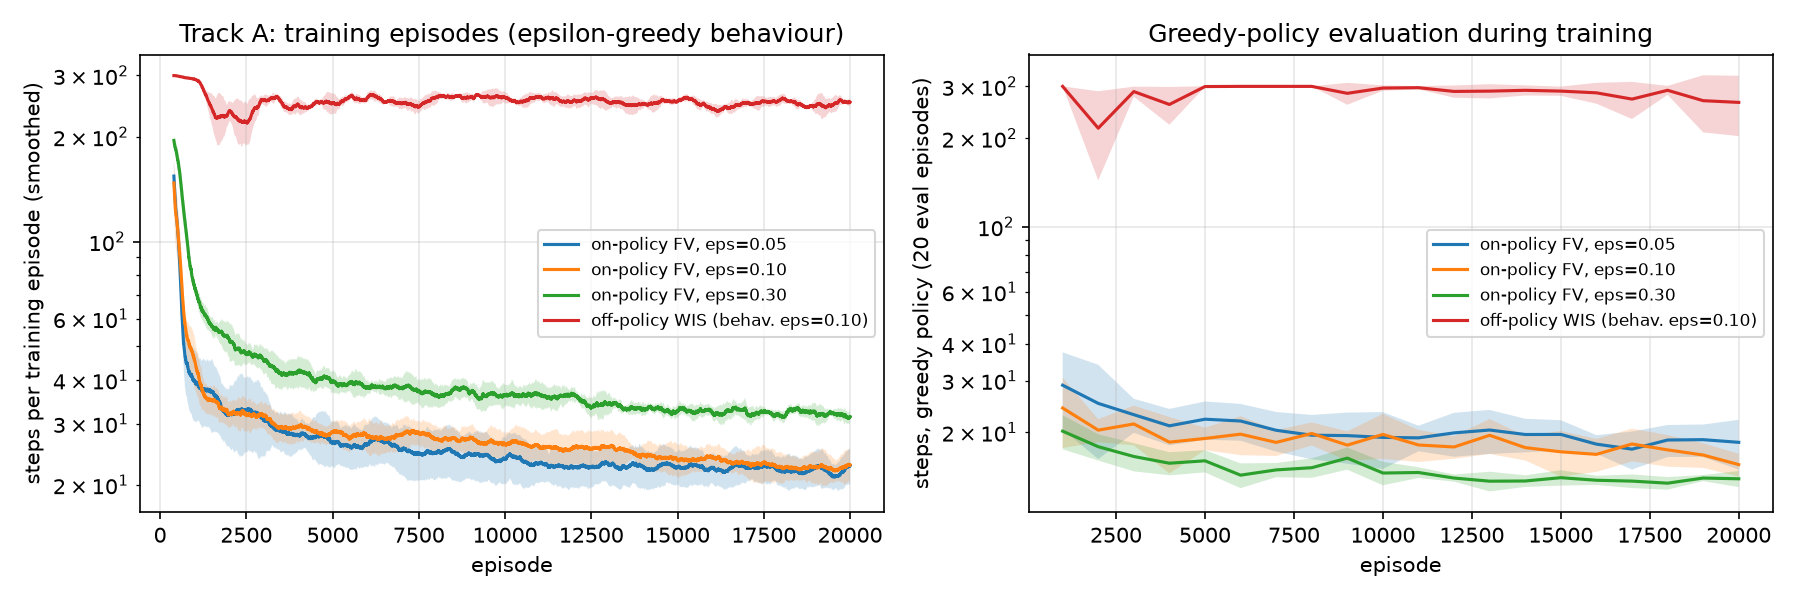
\includegraphics[width=\textwidth]{p1_learning_curves_A.png}
\caption{Track A learning curves (mean $\pm$ sd over 3 seeds, log scale).
\emph{Left:} steps per training episode of the $\varepsilon$-greedy behaviour
policy. \emph{Right:} steps of the greedy policy evaluated
every 1{,}000 episodes.}
\label{fig:p1curves}
\end{figure}

\paragraph{Discussion.}
All on-policy variants drop from several hundred steps to roughly 30--60 steps
per training episode within about 1{,}000--2{,}000 episodes. Amongst the
on-policy variants, $\varepsilon=0.30$ took the longest steps to finish during
training while $\varepsilon=0.10, 0.05$ took similar steps. The trained policy
accelerates along the first straight and cuts the corner toward the finish
(Fig.~\ref{fig:p1traj}).

The exploration rate shows a clear \emph{training vs.\ greedy} trade-off. A
larger $\varepsilon$ costs the agent more steps during training as
shown in the left panel of Fig.~\ref{fig:p1curves}. This is because the agent
is deliberately acting randomly, which causes the agent to take longer time to
complete the race. Once the agent turns off its exploration, its greedy policy
was the fastest in our runs as shown in the right panel of
Fig.~\ref{fig:p1curves}. A plausible explanation is that more exploration visits
more state--action pairs, so the greedy policy of higher $\varepsilon$ is better
estimated.

\begin{figure}[htbp]
\centering
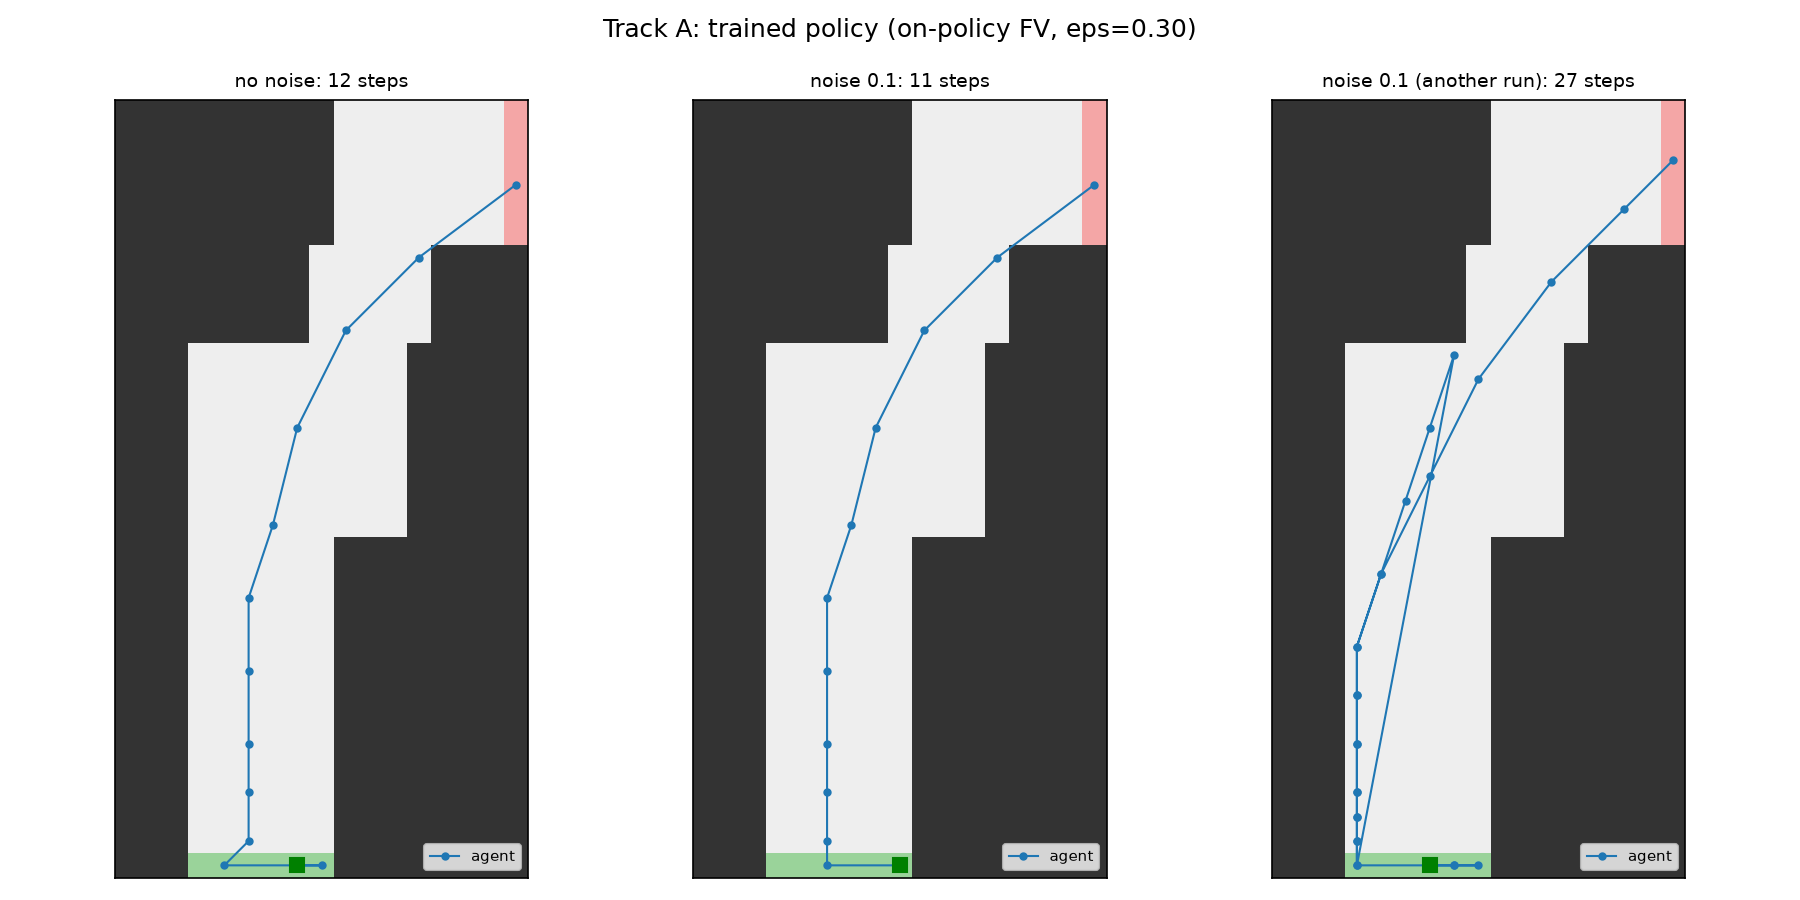
\includegraphics[width=0.85\textwidth]{p1_trajectories_A.png}
\caption{Example runs of a trained policy (the $\varepsilon=0.30$ on-policy agent, 
seed 0). Green represents start cell of the run while pink represents finish line. 
Left figure shows that no environment noise was added while middle and right shows 
added noise of $0.1$. In the middle panel the car crashes shortly after the start, 
is reset, and still finishes.}
\label{fig:p1traj}
\end{figure}

Off-policy weighted Importance Sampling MC learned far more slowly. after
20{,}000 episodes the greedy policy still often hit the 300 steps to complete
the race. A likely cause is due to the stops in the backward update at the last
non-greedy action. Therefore, only a few time steps of each episode contributes
to learning for long episodes with a soft behaviour policy. 

\section{Part 2: Multi-agent racetrack}
\paragraph{Setup.} A second car runs on the same track following the
\emph{greedy} Part~1 policy (the $\varepsilon=0.30$ agent, seed 0), under the
same dynamics and noise. A \emph{collision} occurs when the cells swept by the
two cars in one time step intersect. If the two cars collide, the agent respawns
at the start after a crash and pays an extra penalty of $10$ on top of the $-1$
step cost. 

\paragraph{Three different modes the agent can observe}
\begin{itemize}
\item \textbf{none}: nothing about the other car (state unchanged).
\item \textbf{pos}: the opponent's position relative to the learner, $(\Delta
r,\Delta c)$, if within a $7\times7$ window (radius 3), otherwise a single
``far/absent'' value.
\item \textbf{posvel}: as \textbf{pos} plus one flag indicating whether the
opponent's speed is at least 2. (speed $\ge2$)
\end{itemize}
The \textbf{opponent start offset} is varied: $0$ (both start together), $+6$
(opponent waits 6 steps, so it chases the learner), $-6$ (opponent gets a 6-step
head start). This gives $3\times3=9$ conditions, each trained with on-policy
first-visit MC ($\varepsilon=0.05$).

\begin{figure}[htbp]
\centering
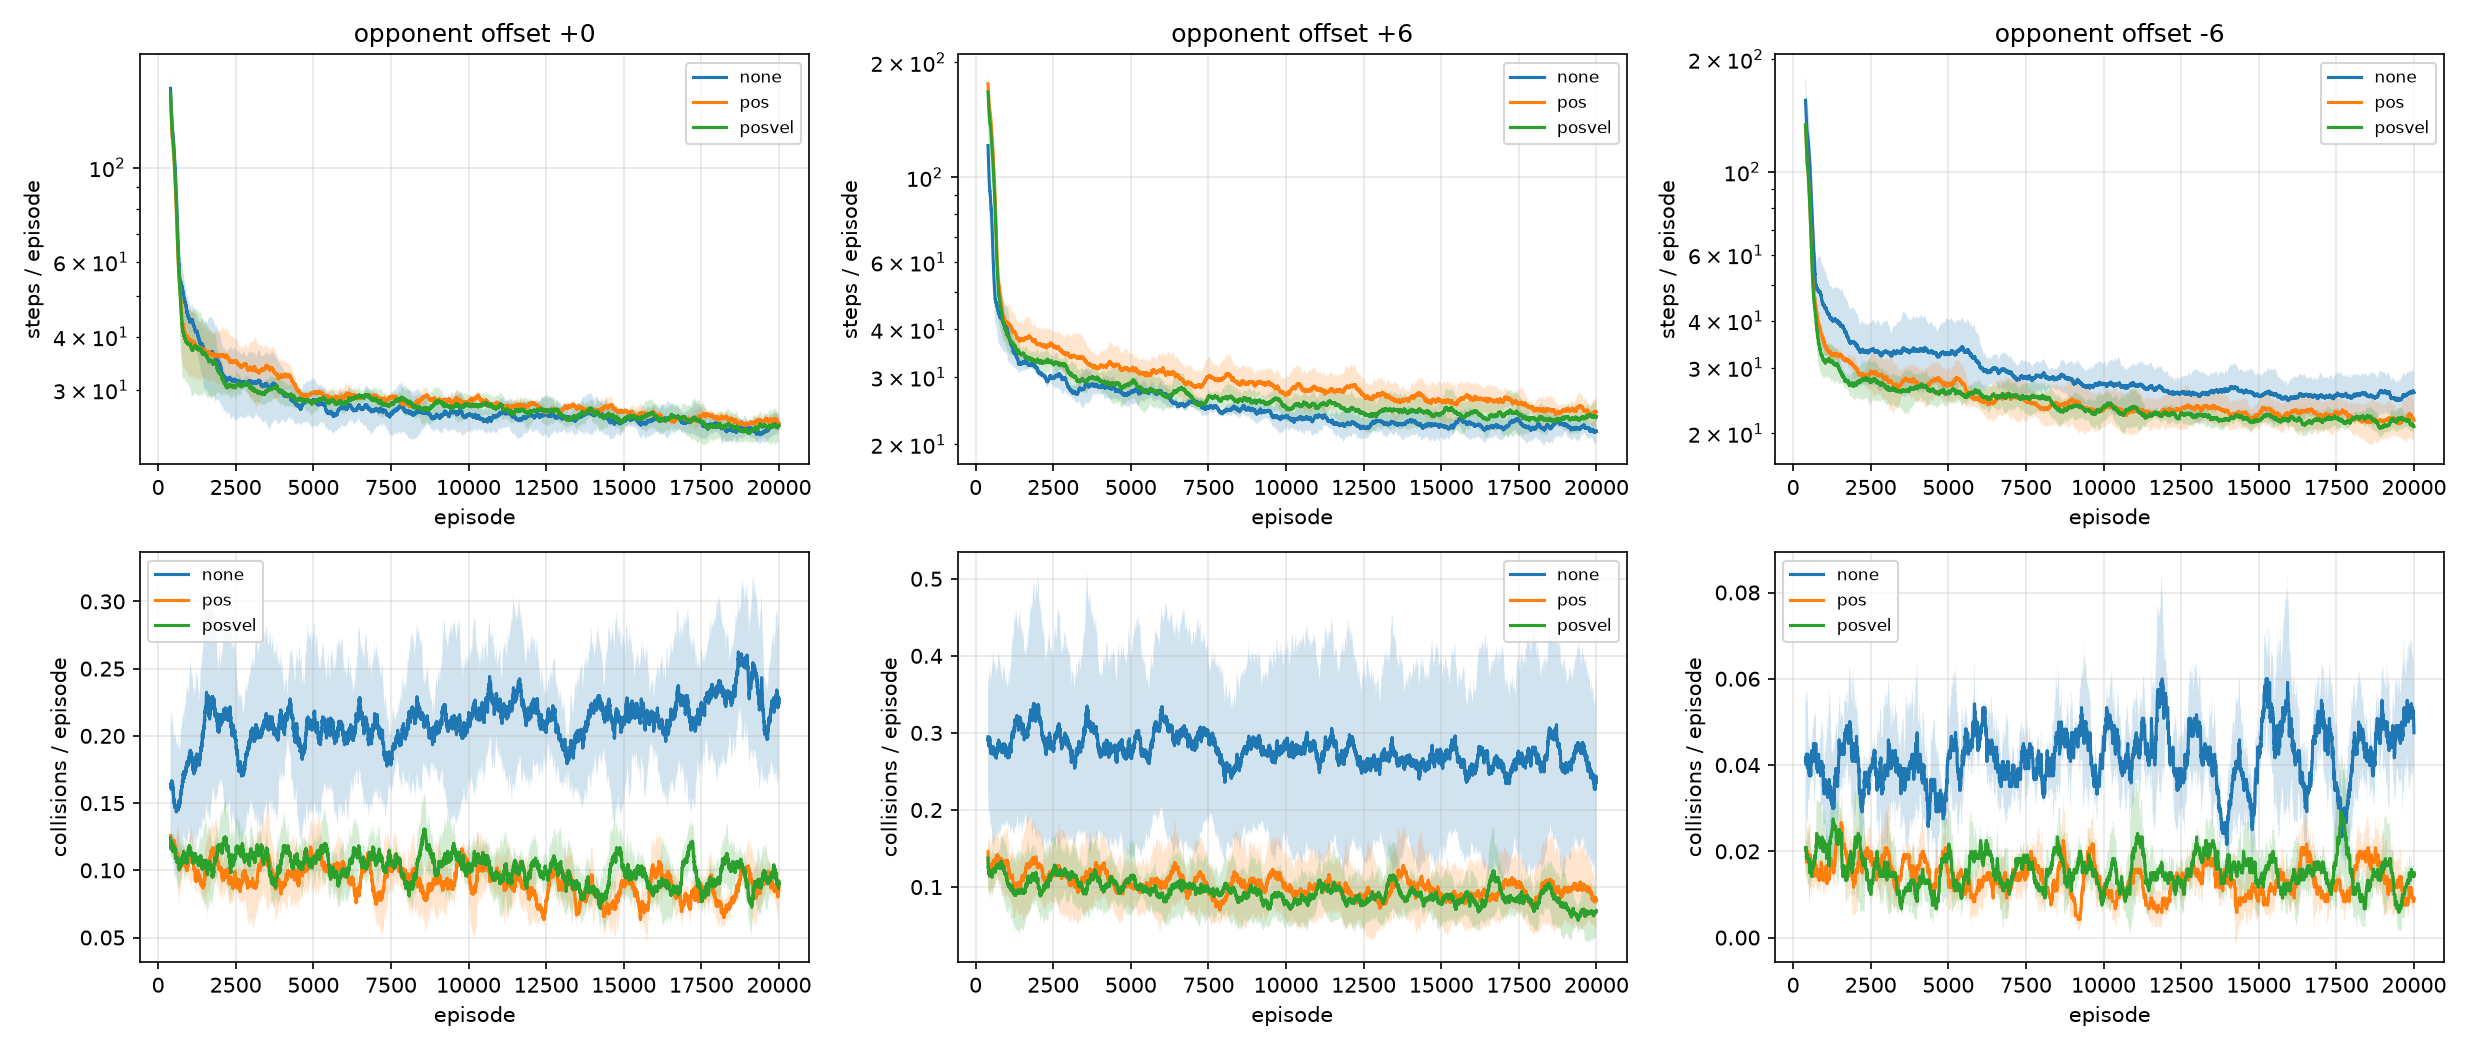
\includegraphics[width=\textwidth]{p2_learning_curves_A.png}
\caption{Part 2 learning curves (mean $\pm$ sd over 3 seeds). Top graphs show steps per training episode and bottom graphs show collisions per training episode. Each columns represent opponent offsets and observation type.}
\label{fig:p2curves}
\end{figure}

\paragraph{Discussion.}
\emph{Collisions.} Seeing the other car's relative position reduces collisions
substantially in every offset condition: from around 0.2 to 0.1 per episode at
offset 0, from around 0.3 to 0.1 at $+6$, and from around 0.05 to 0.01 at $-6$.
Another feature of the collision curves in Fig.~\ref{fig:p2curves} is that the
blind agent's curves are noticeably noisier across seeds. A blind agent can only
learn a policy that is good on average against where the opponent usually is, but an
agent that sees the opponent can slow down or change lane when it is close.

\emph{Speed.} All agents finish every episode. Differences in steps are small
compared with the seed-to-seed standard deviation (about 1--3 steps). One thing
to notice is that when opponent waits 6 steps before it starts (offset $+6$),
agent with no information on opponent completed race slightly faster than agent
with positional and speed information. When agent waits 6 steps before it
starts, on the other hand, the blind agent was the slowest to finish the race on
average. 

\emph{Does velocity help?} The \textbf{posvel} agent was not clearly better than
\textbf{pos} in any offset condition. Both agents on required similar steps to
complete the episode (top chart) and the number of collisions (bottom chart)
show similar performance. This might be because the flag information is not very
useful: the opponent's speed is already reflected in its position, and the agent
can learn to infer speed from the opponent's position over time.

\emph{Caveats.} The opponent is a fixed, non-reactive policy, so the problem
remains close to a single-agent MDP with a moving obstacle. A reactive or
learning opponent would make the environment non-stationary and violate the
assumptions behind MC convergence.

\begin{figure}[htbp]
\centering
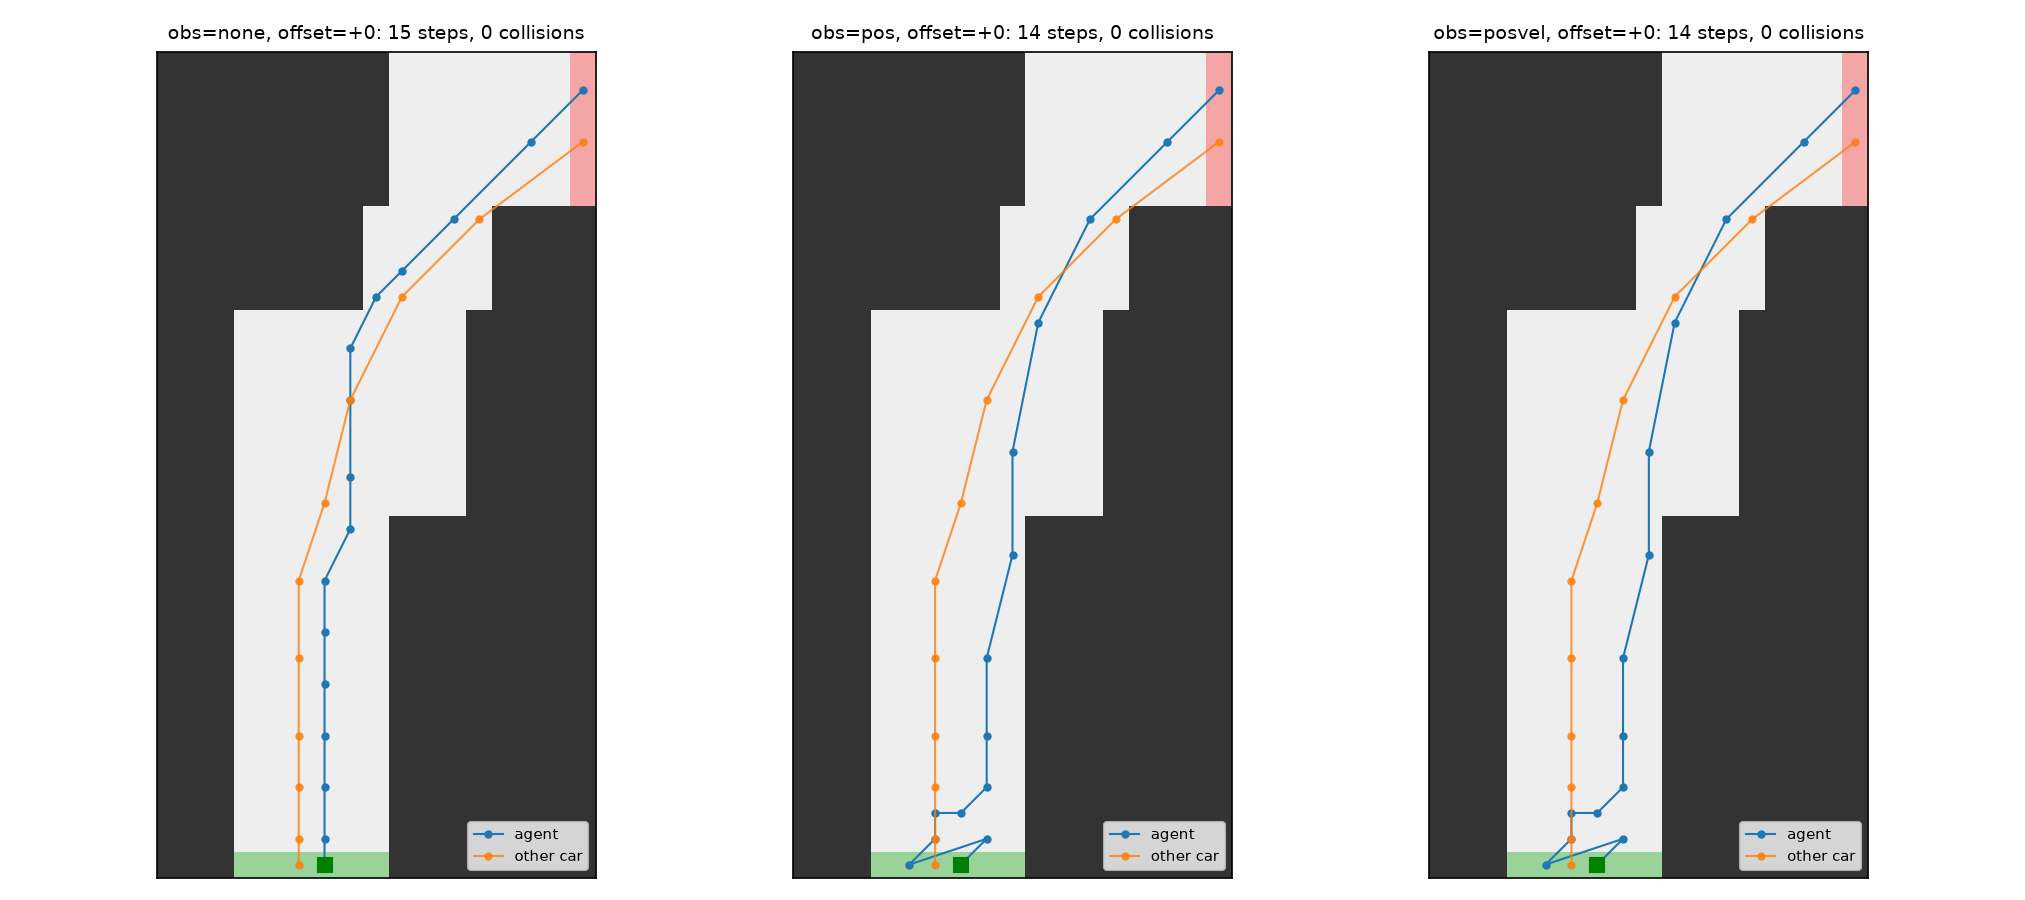
\includegraphics[width=\textwidth]{p2_trajectories_A.png}
\caption{Example runs of trained agents with different modes (offset 0, seed 0). 
The agent is represented in blue and opponent car is represented in orange.}
\label{fig:p2traj}
\end{figure}

\section{Part 3: Windy Prize Race}
\subsection{Environment design}
A $7\times10$ grid world is implemented with random wind columns and prize at
random location. The car starts in the bottom-left corner (\textbf{S}) and must
reach the bottom-right corner
(\textbf{G}). Three features make the problem non-trivial:
\begin{itemize}
\item \textbf{Wind.} There are three columns, chosen at random (never the start
or goal column) that blow \emph{upward}. When agent lands on a windy column, it
is carried up by $k$ cells, where $k$ is drawn uniformly from
$\{0,\dots,k_{\max}\}$ (default $k_{\max}=2$).
\item \textbf{Prize.} One prize lies in a randomly chosen cell and is picked up
automatically when the agent lands on the prize cell. When the prize is
collected, the agent receives a reward $+5$.
\item \textbf{Mandatory pickup.} The race only finishes when the agent enters
the goal cell \emph{holding the prize}. When agent successfully completes the
race with the prize, it receives a reward $+20$.
\end{itemize}
Every step costs $-1$. Actions are up/down/left/right; moving into the border
leaves the agent where it is. The windy columns and the prize cell are drawn
once when an environment is created and then stay fixed.
The only randomness within an episode is the wind strength. The state is (row,
column, has\_prize), which would be 140 states and 4 actions.

\subsection{Is it solvable by MC?}
MC control needs complete episodes, and here the episode ends only when the
agent finishes the race. That is not guaranteed: a policy that never collects
the prize or loops forever never terminates. Therefore, the experiment uses
truncated episodes at 200 steps and its return for learning. Truncated returns
depend on \emph{when} in an episode a state was first visited, which biases
value estimates for states in loops.

In addition, the reward is sparse in the sense that the agent has to find a
specific sequence (prize, then goal) before anything positive happens, and MC
only updates state--action pairs it actually visits. Therefore, it is expected
that MC to be workable but sensitive to exploration.

\subsection{Experiment design}
All experiments are conducted over 5{,}000 training episodes,
with a maximum of 200 steps per episode and a discount factor
of $\gamma = 1$. The greedy policy is evaluated on 30 episodes
every 250 training episodes, followed by a final evaluation
over 200 episodes.

To account for variability across runs, each experiment is
repeated with 8 random seeds. A seed is considered
\emph{solved} if its learned greedy policy successfully
completes at least 90\% of the 200 final evaluation episodes.
We report the number of solved seeds out of 8, along with
the mean final greedy return and standard deviation across
solved seeds only. The optimal return obtained through
value iteration is included as a reference.

Unless otherwise specified, ``MC return'' refers to the
mean final greedy return across solved seeds.

\subsection{Experiment on wind strength}
The maximum wind $k_{\max}\in\{0,1,2,3\}$ was applied on two layouts: layout~0
with wind has no effect on the optimum and layout~9 with windy columns 3, 7, 8;
prize at row 4, column 1. There was a noticable drop of the optimal return from
$12.0$ to $8.5$ when stronger wind exist.

\begin{figure} \centering
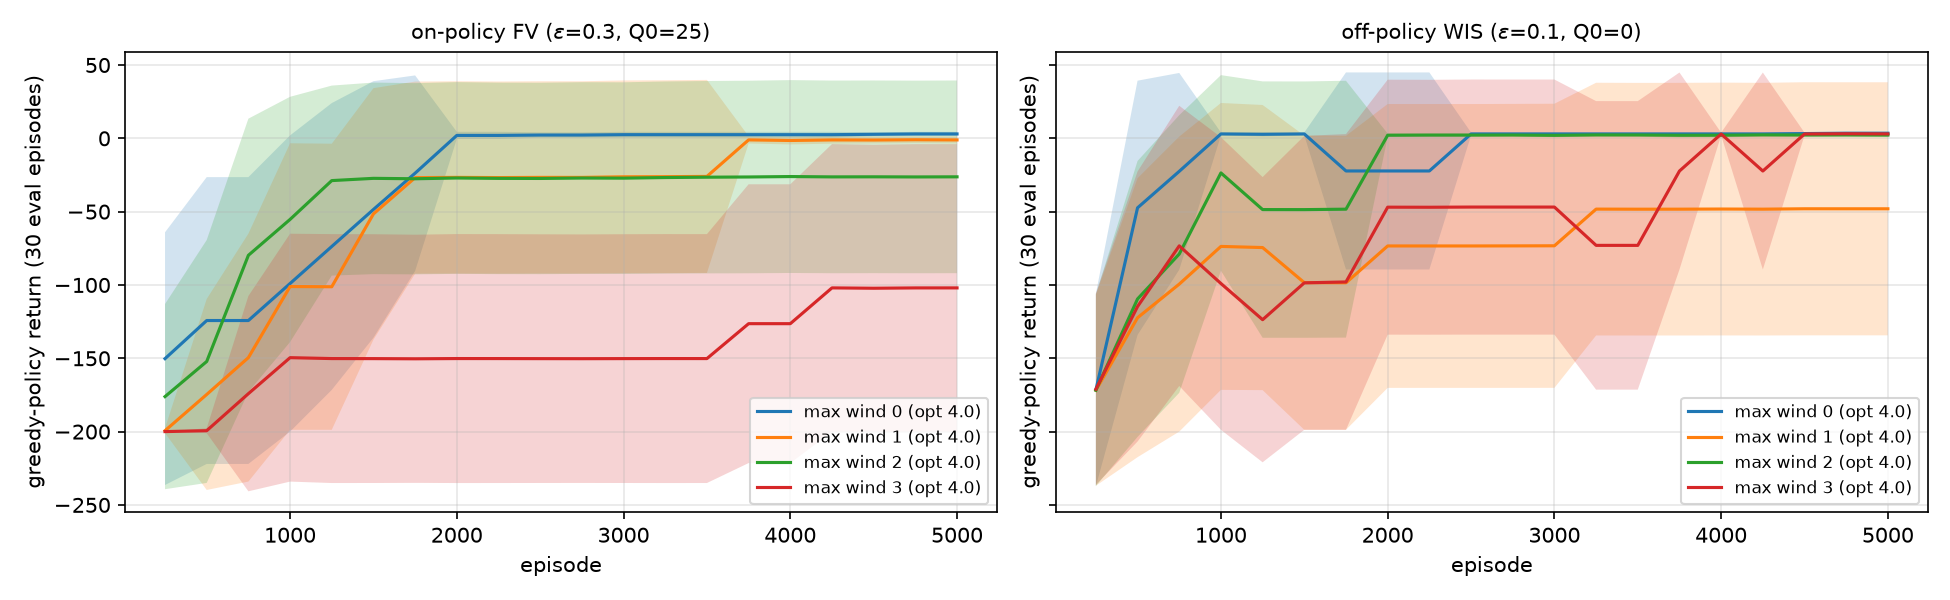
\includegraphics[width=\textwidth]{p3_expB_wind_L0.png} 
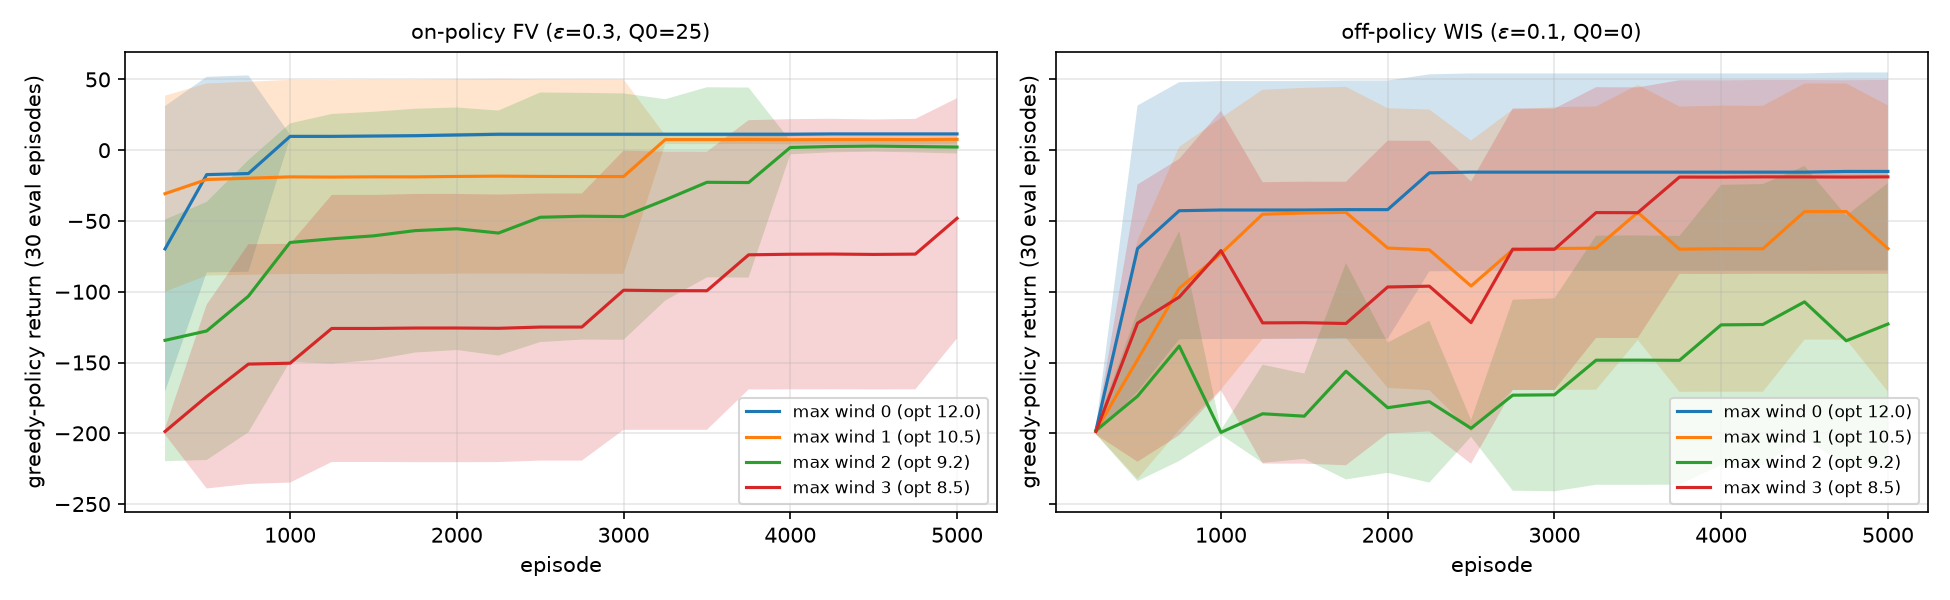
\includegraphics[width=\textwidth]{p3_expB_wind_L9.png} 
\caption{Top figures represent layout 0 (8 seeds): mean greedy-policy return during
training for each wind strength. Bottom figures represent layout 0. The mean
includes the seeds that never finish.} 
\label{fig:p3B} 
\end{figure}

\paragraph{Discussion.} The wind makes MC
harder for two plausible reasons: the return of a state--action pair
becomes much noisier with large standard deviations across seeds, and random
exploration is blown around, making the prize-then-goal sequence harder to find.
Since the optimal return does not change with wind, the loss in performance here
comes from learning difficulty rather than from a harder optimal task.
Off-policy results were less monotonic (e.g.\ 3/8 solved at $k_{\max}=2$ but 7/8
at $k_{\max}=3$ on layout~9), which can be interpreted as noise and
sensitivity to the specific seeds rather than a real effect of wind.

\begin{figure}
\centering
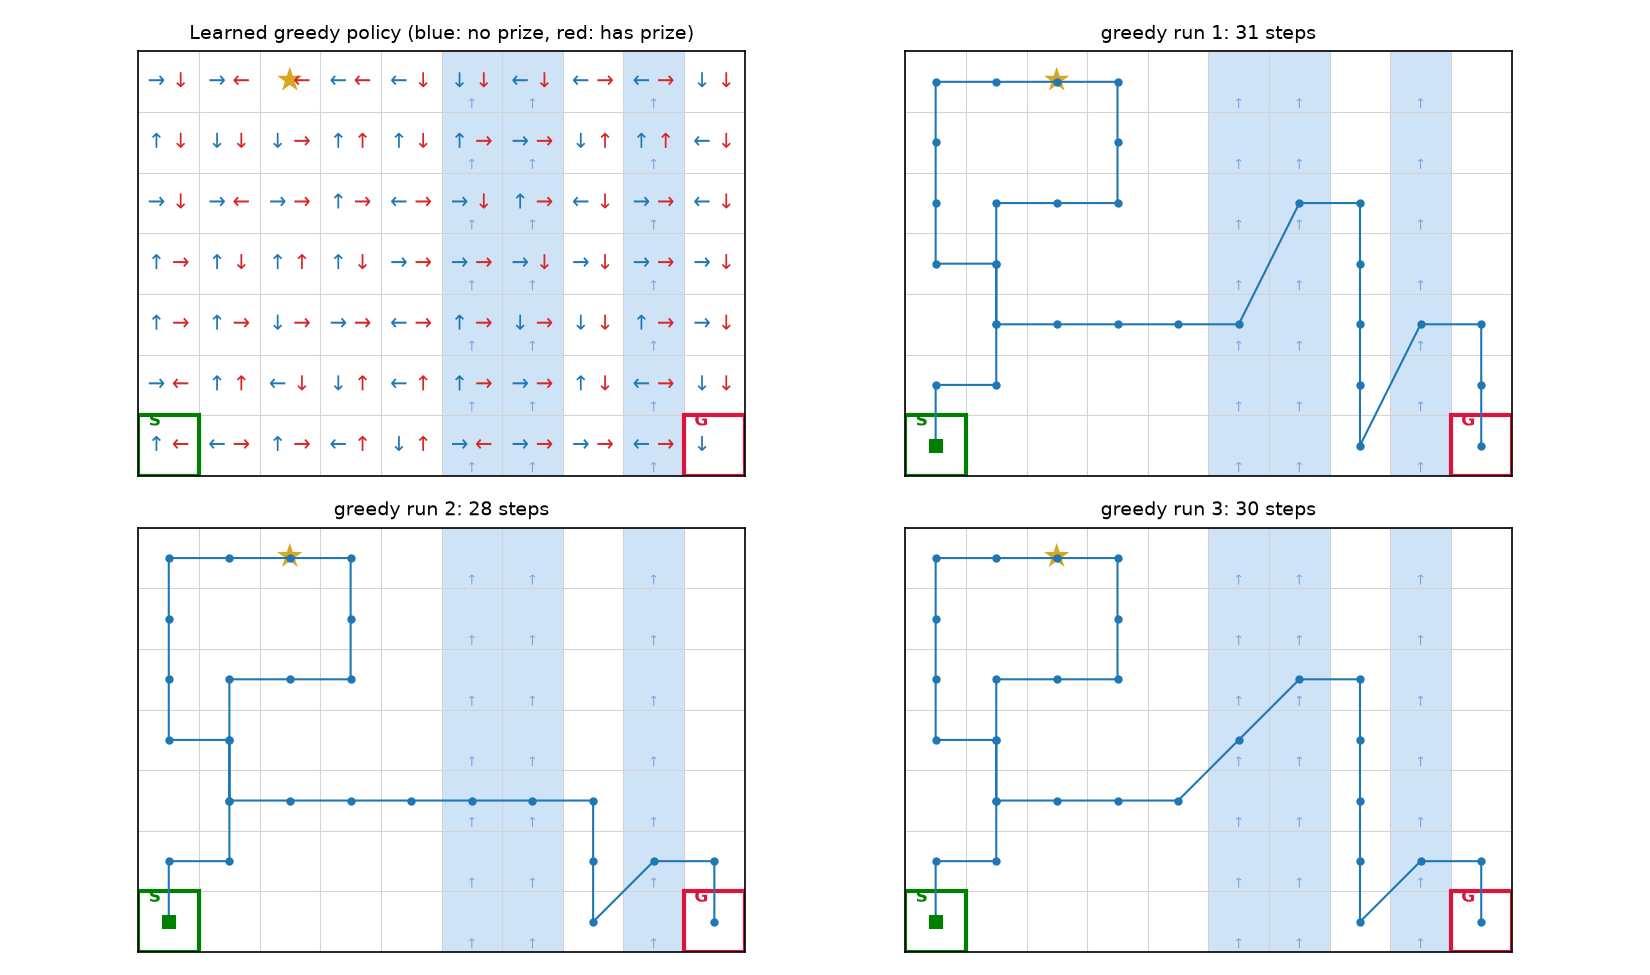
\includegraphics[width=0.95\textwidth]{p3_policy.png}
\caption{Figures are all from layout 0. Top left represents greedy policy with 
blue showing moves for prize not yet held and red showing for prize held. The 
shaded columns are windy, the star is the prize. Other three panels illustrate
three greedy runs with different wind draws. The lines through windy columns 
show the agent being carried upward.}
\label{fig:p3pol}
\end{figure}

\subsection{Example policy}
Figure~\ref{fig:p3pol} shows the greedy policy and three runs for one
first-visit agent. The agent picks up the prize in the top row and
then reaches the goal, but it does so via a long detour of 28--31 steps rather
than the optimal 21. Arrows are drawn for every state with at least one visit.
With optimistic initialisation, every state is visited early on. Therefore, arrows in
rarely visited states rest on very few samples.

\section{Conclusions}
The racetrack example was implemented with Monte Carlo method in this report.
The on-policy $\varepsilon$-soft MC solves the racetrack in a few thousand
episodes, whereas off-policy weighted-IS MC with a soft behaviour policy is much
slower on this task. With the small grid world implementation, it still works
well. In part 2, another car was added to examine learners behaviour. Giving the
learner the other car's relative position substantially reduces collisions, but
the speed flag did not help agent to learn. In a newly created grid world with
wind and prize setup, Monte Carlo method is usable
only after making termination and penalties compatible with truncated episodes.

\section{Extra Credit}
\paragraph{Exercise 5.11}
W update involves the importance-sampling ratio \(1 \over b(A_t\mid S_t)\)
instead of \(\pi(A_t\mid S_t) \over b(A_t\mid S_t)\). This is because the
algorithm only updates when the behavior action matches the target policy's
action. Since the target policy is deterministic and greedy, its values are
either 1 or 0. When the actions match, \(\pi(A_t\mid S_t)=1\), and the
importance-sampling ratio simplifies to \(1/b(A_t\mid S_t)\). When the actions
differ, \(\pi(A_t\mid S_t)=0\), and the algorithm terminates the loop. Thus, the
algorithm implicitly accounts for the numerator of the importance-sampling
ratio.

\paragraph{Exercise 6.1}
Equation (6.6) states that the Monte Carlo error can be expressed as the
discounted sum of TD errors:
\[
G_t - V(S_t)
= \sum_{k=t}^{T-1} \gamma^{k-t}\delta_k.
\]
However, this equality assumes that the value function remains unchanged
throughout the episode.

When the value function changes over time, the TD error at time $k$ becomes
\[
\delta_k
= R_{k+1} + \gamma V_k(S_{k+1}) - V_k(S_k).
\]

Expanding the discounted sum of TD errors gives
\begin{align*}
\sum_{k=t}^{T-1}\gamma^{k-t}\delta_k
&= \sum_{k=t}^{T-1}\gamma^{k-t}R_{k+1} \\
&\quad + \sum_{k=t}^{T-1}
    \gamma^{k-t+1}V_k(S_{k+1}) \\
&\quad - \sum_{k=t}^{T-1}
    \gamma^{k-t}V_k(S_k).
\end{align*}

Since
\[
G_t = \sum_{k=t}^{T-1}\gamma^{k-t}R_{k+1},
\]
and the terminal state has value zero, we can rearrange the terms:
\begin{align*}
\sum_{k=t}^{T-1}\gamma^{k-t}\delta_k
&= G_t - V_t(S_t) \\
&\quad + \sum_{k=t+1}^{T-1}\gamma^{k-t}
\left[V_{k-1}(S_k)-V_k(S_k)\right].
\end{align*}

Rearranging to isolate the Monte Carlo error:
\[
{
\begin{aligned}
G_t - V_t(S_t)
&= \sum_{k=t}^{T-1}\gamma^{k-t}\delta_k \\
&\quad + \sum_{k=t+1}^{T-1}\gamma^{k-t}
\left[V_k(S_k)-V_{k-1}(S_k)\right].
\end{aligned}
}
\]

Therefore, the additional correction term is
\[
\boxed{
\sum_{k=t+1}^{T-1}\gamma^{k-t}
\left[V_k(S_k)-V_{k-1}(S_k)\right].
}
\]

This correction accounts for changes in the value function between consecutive
time steps. When the value function remains constant, the correction term
becomes zero, and Equation (6.6) holds exactly.

\end{document}